%
% msa.tex -- visual representation of MSA
%
% (c) 2019 Prof Dr Andreas Müller, Hochschule Rapperswil
%
\documentclass[tikz]{standalone}
\usepackage{amsmath}
\usepackage{times}
\usepackage{txfonts}
\usepackage{pgfplots}
\usepackage{csvsimple}
\usetikzlibrary{arrows,intersections,math,fadings,shadings}
\begin{document}
\def\Fs{\textit{fs}}
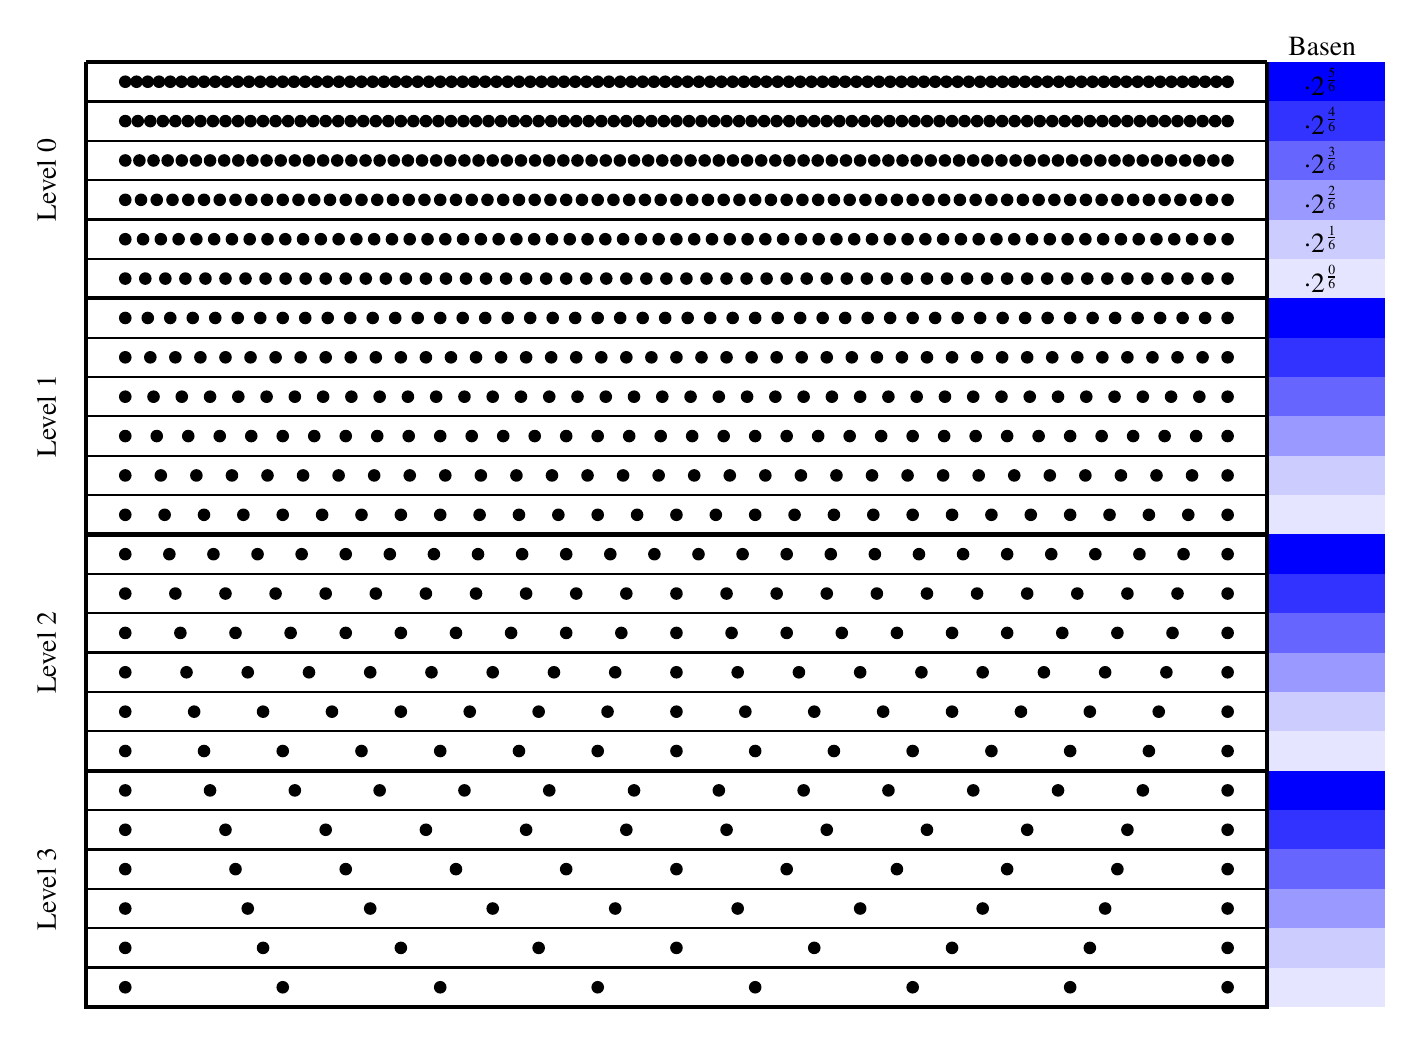
\begin{tikzpicture}


\draw (-0.5,-1.5) node[rotate=90]{Level 0};
\draw (-0.5,-4.5) node[rotate=90]{Level 1};
\draw (-0.5,-7.5) node[rotate=90]{Level 2};
\draw (-0.5,-10.5) node[rotate=90]{Level 3};



\draw (15.7,0.2) node{Basen};

\foreach \x in {0,-3,...,-11}{
	
	\fill [blue!100!white] (15.0,\x-0.5) rectangle (16.5,\x);
	
	\fill [blue!80!white] (15.0,\x-1) rectangle (16.5,\x-0.5);
	
	\fill [blue!60!white] (15.0,\x-1.5) rectangle (16.5,\x-1);
	
	\fill [blue!40!white] (15.0,\x-2) rectangle (16.5,\x-1.5);
	
	\fill [blue!20!white] (15.0,\x-2.5) rectangle (16.5,\x-2);
	
	\fill [blue!10!white] (15.0,\x-3) rectangle (16.5,\x-2.5);
	
}
	\draw (15.7,-0.25) node{$\Fs\cdot2^{\frac{5}{6}}$};
	\draw (15.7,-0.75) node{$\Fs\cdot2^{\frac{4}{6}}$};
	\draw (15.7,-1.25) node{$\Fs\cdot2^{\frac{3}{6}}$};
	\draw (15.7,-1.75) node{$\Fs\cdot2^{\frac{2}{6}}$};
	\draw (15.7,-2.25) node{$\Fs\cdot2^{\frac{1}{6}}$};
	\draw (15.7,-2.75) node{$\Fs\cdot2^{\frac{0}{6}}$};
\draw[ultra thick] (0,0)--(0,-12)--(15,-12)--(15,0);

\foreach \x in {0,-3,...,-12}{
	\draw[ultra thick] (0,\x)--(15,\x);
}



\foreach \x in {0,-0.5,...,-12}{
	\draw[thick] (0,\x)--(15,\x);
}

\foreach \k/\y in {98/-0.25,88/-0.75,78/-1.25,70/-1.75,62/-2.25,55/-2.75}{
	\pgfmathparse{0.5+14/\k}
	\xdef\s{\pgfmathresult}
	\foreach \x in {0.5,{\s},...,14.5}{
		\fill({\x},\y) circle[radius=0.08];
	}
}


\foreach \k/\y in {49/-3.25,44/-3.75,39/-4.25,35/-4.75,31/-5.25,28/-5.75}{
	\pgfmathparse{0.5+14/\k}
	\xdef\s{\pgfmathresult}
	\foreach \x in {0.5,{\s},...,14.5}{
		\fill({\x},\y) circle[radius=0.08];
	}
}

\foreach \k/\y in {25/-6.25,22/-6.75,20/-7.25,18/-7.75,16/-8.25,14/-8.75}{
	\pgfmathparse{0.5+14/\k}
	\xdef\s{\pgfmathresult}
	\foreach \x in {0.5,{\s},...,14.5}{
		\fill({\x},\y) circle[radius=0.08];
	}
}

\foreach \k/\y in {13/-9.25,11/-9.75,10/-10.25,9/-10.75,8/-11.25,7/-11.75}{
	\pgfmathparse{0.5+14/\k}
	\xdef\s{\pgfmathresult}
	\foreach \x in {0.5,{\s},...,14.5}{
		\fill({\x},\y) circle[radius=0.08];
	}
}

\end{tikzpicture}
\end{document}

